% ****** Start of file apssamp.tex ******
%
%   This file is part of the APS files in the REVTeX 4.1 distribution.
%   Version 4.1r of REVTeX, August 2010
%
%   Copyright (c) 2009, 2010 The American Physical Society.
%
%   See the REVTeX 4 README file for restrictions and more information.
%
% TeX'ing this file requires that you have AMS-LaTeX 2.0 installed
% as well as the rest of the prerequisites for REVTeX 4.1
%
% See the REVTeX 4 README file
% It also requires running BibTeX. The commands are as follows:
%
%  1)  latex apssamp.tex
%  2)  bibtex apssamp
%  3)  latex apssamp.tex
%  4)  latex apssamp.tex
%
\documentclass[%
 reprint,
 superscriptaddress,
%groupedaddress,
%unsortedaddress,
%runinaddress,
%frontmatterverbose, 
%preprint,
%showpacs,preprintnumbers,
%nofootinbib,
%nobibnotes,
%bibnotes,
 amsmath,amssymb,
 %aps,
pra,
%prb,
%rmp,
%prstab,
%prstper,
%floatfix,
]{revtex4-1}

\usepackage{graphicx}% Include figure files
\usepackage{dcolumn}% Align table columns on decimal point
\usepackage{cancel}
\usepackage{tikz}
\usepackage{pgfplots}
\pgfplotsset{compat=1.13}
\setcitestyle{square}

\usepackage{bm}% bold math
\usepackage{verbatim}
%\usepackage{hyperref}% add hypertext capabilities
%\usepackage[mathlines]{lineno}% Enable numbering of text and display math
%\linenumbers\relax % Commence numbering lines

%\usepackage[showframe,%Uncomment any one of the following lines to test 
%%scale=0.7, marginratio={1:1, 2:3}, ignoreall,% default settings
%%text={7in,10in},centering,
%%margin=1.5in,
%%total={6.5in,8.75in}, top=1.2in, left=0.9in, includefoot,
%%height=10in,a5paper,hmargin={3cm,0.8in},
%]{geometry}

\begin{document}

%\preprint{APS/123-QED}

%\thanks{A footnote to the article title}%
\title{Homework Title}

\author{Your Name}
\email{yourname@tum.de}
\affiliation{%
 Department of Electrical and Computer Engineering, Technical University of Munich, Arcisstra{\ss}e 21, 80333 Munich, Germany
}%

\date{\today}% It is always \today, today,
             %  but any date may be explicitly specified

\begin{abstract}
Please use this \LaTeX{} template to structure your report. The structure below is commonly used for scientific paper writing. We recommend to try to keep to this structure in order to practice scientific writing. Please do not exceed 4 pages, additional information like parts of the code can be added in the appendix (does not count to the 4 pages).
\end{abstract}

\pacs{Valid PACS appear here}% PACS, the Physics and Astronomy
                             % Classification Scheme.
%\keywords{Suggested keywords}%Use showkeys class option if keyword
                              %display desired
\maketitle

%\tableofcontents


\section{Introduction}
\label{sec:introduction}

Why do we care about the problem and the results?  This section should include the importance of your work (the discussed topic), the difficulty of the area, and the impact it might have if successful.

What problem are you trying to solve? What is the scope of your work (a generalized approach, or for a specific situation)? 


\section{Methods}
\label{sec:methods}

How did you go about solving or making progress on the problem? Did you use simulation, analytic models, prototype construction, or analysis of field data for an actual product? What was the extent of your work (did you look at one application program or a hundred programs in twenty different programming languages?) What important variables did you control, ignore, or measure?

\subsection*{Example Equation}
In Born-Oppenheimer approximation, the electron and nuclei motion is separated. The Hamiltonian of a many-particle system, e.g. a molecule, is given by
\begin{equation}
\label{eq:example_equation}
    \hat{H} = \sum_i \frac{\hbar^2}{2m}\nabla_i^2 - \sum_{i<j}\frac{e^2}{r_{ij}} + \sum_{i}\sum_{k}\frac{e^2 Z_{k}}{r_{ij}} \,,
\end{equation}
where $\hbar$ is the reduced Planck's constant, $m$ is the electron mass, \dots 

We can refer to the example equation using the reference command: See eq. (\ref{eq:example_equation}).

\section{Results}
\label{sec:results}

What's the answer? Put the result there, in numbers. Plot your results including all important facts, label the axis, show a legend, and give an explanation to the obtained results.

\subsection*{Example Figure}

In Fig. \ref{fig:C60_molecular_orbitals} the molecular orbitals for the C60 molecule are shown. 

\begin{figure}[h]
    \centering
    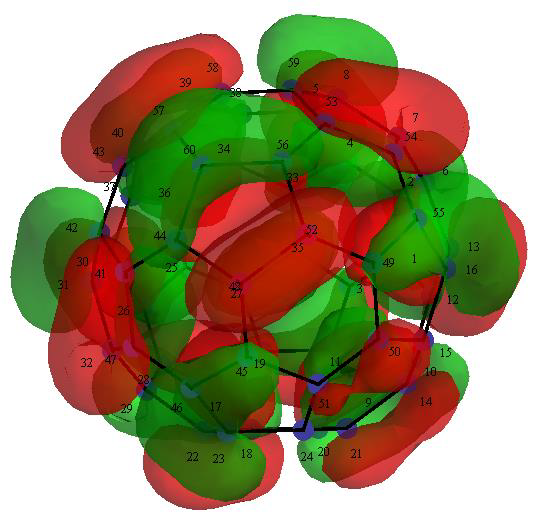
\includegraphics[width=\columnwidth]{grafik/MO_LUMO_C60.png}
    \caption{Molecular orbitals of the C60 bucky ball molecule.}
    \label{fig:C60_molecular_orbitals}
\end{figure}

\subsection*{Example Citation}

An introduction to quantum mechanics is given by \cite{griffiths2016introduction}.

\section{Conclusion}
\label{sec:conclusion}
What are the implications of your answer? Are your results general, potentially generalizable, or specific to a particular case?

\section*{Appendix}
Additional information and codes.

\bibliographystyle{apsrev4-1}
\bibliography{references}

% \pagebreak

\end{document}
%
% ****** End of file apssamp.tex ******
